% This is samplepaper.tex, a sample chapter demonstrating the
% LLNCS macro package for Springer Computer Science proceedings;
% Version 2.20 of 2017/10/04
%
\documentclass[runningheads]{llncs}
%
\usepackage{graphicx}
% Used for displaying a sample figure. If possible, figure files should
% be included in EPS format.
%
% If you use the hyperref package, please uncomment the following line
% to display URLs in blue roman font according to Springer's eBook style:
% \renewcommand\UrlFont{\color{blue}\rmfamily}
\usepackage[utf8]{inputenc}

\begin{document}
%
\title{Towards Initial Understanding of Human Behavior During Typhoon Evacuation: An Application of Agent-Based Modeling} %\thanks{Supported by organization x.}}

%
%\titlerunning{Abbreviated paper title}
% If the paper title is too long for the running head, you can set
% an abbreviated paper title here
%
\author{Rey C. Rodrigueza\inst{1,3}\orcidID{0000-0002-8892-4288} \and
Kevin Chapuis\inst{2}\orcidID{1111-2222-3333-4444} \and
Maria Regina Justina E. Estuar\inst{1}\orcidID{2222--3333-4444-5555}}
%
\authorrunning{F. Author et al.}
% First names are abbreviated in the running head.
% If there are more than two authors, 'et al.' is used.
%
\institute{Ateneo Social Computing Science Laboratory,\\Department of Information Systems and Computer Science,\\
    Ateneo de Manila University, Quezon City, Philippines 1108\\
    %\email{\{rey.rodrigueza,res\}@uni-heidelberg.de}
    \and
IRD-UMMISCO\\
\email{lncs@springer.com}\\
%\url{http://www.springer.com/gp/computer-science/lncs} \and
Department of Information and Communications Technology\\Sorsogon State College - Bulan Campus, Bulan, Sorsogon, Philippines 4706\\
\email{rcrodrigueza@gmail.com}}
%
\maketitle              % typeset the header of the contribution
%
\begin{abstract}
Natural disasters continue to cause tremendous damage to humans' lives and properties. The Philippines, due to its geographic location, is considered a natural disaster-prone country experiencing an average of 20 tropical cyclones annually. This condition necessitates the need to study what can be done to mitigate the effects of weather-related disaster. Understanding human behavior during disasters could help in making decisions on how to prepare for disasters, how to act appropriately and strategically respond during and after a calamity. In this paper, an agent-based model of human behavior during typhoon evacuation is presented. In the model, civilians are represented by households and their evacuation decisions were based from their calculated perceived risk. Also, rescuer and shelter manager agents were included as facilitators during the evacuation process. Further, geospatial data of a village in a typhoon-susceptible municipality was used to represent the environment. Finally, the number of households who decided to evacuate or opted to stay as influenced by the model’s decision factors were determined during simulations.

\keywords{agent-based modeling  \and typhoon evacuation \and human behavior.}
\end{abstract}
%
%
%
\section{Introduction}
[DRAFT] Disasters are exacting an enormous damage with hundreds of thousands of lives and US\$1.5 trillion lost in the last decade alone \cite{unisdr2015report}. In 2017, a total of 335 natural disasters affected more than 96.6 million people, and further 9,697 casualties with damages amounting to US \$335 billion \cite{annualdisasterstatisticalreview2017}. Asia appears to be the mostly affected continent as in all disaster events, 44\% of it were caused by storms and floods which took 58\% of the total deaths and 70\% of the people affected \cite{annualdisasterstatisticalreview2017}. 

 United Nations International Strategy for Disaster Reduction (UNISDR) acknowledges that behavioural change of society is needed to significantly diminish disaster losses \cite{unisdr2016framework}. Major changes in attitudes and behaviours towards disaster risk reduction are now indicated and elaborated more in all the recent international agreements (SAMOA Pathway, Sendai Framework for Disaster Risk Reduction 2015 - 2030, Addis Adaba Action Agenda on financing for development, the Paris Agreement on climate change and the New Urban Agenda) \cite{unisdr2016framework}. 
 
 According to World Risk Index 2018 \cite{worldriskreport2018}, the Philippines is the third country in the world with the highest disaster risk, following Vanuatu and Tonga. These three island nations including twelve others have a very high exposure to extreme natural events like typhoons or earthquakes, and coincidentally have extreme level of societal vulnerability. Another study \cite{inform2019} also ranked Philippines as third in the world when it comes to hazard risk and exposure.

The Philippines is a disaster-prone country (ranked 4th in the world according to U.N., 2015) and among the top 10 countries with the highest absolute number of affected people \cite{humanCost}. Its natural geographic location and physical environment make it vulnerable to typhoons, floods, volcanic eruptions, storm surges, earthquakes, tsunamis and drought. As a matter of fact, almost all population in the Philippines is potentially exposed to tropical cyclone wind (99\%) of which 79\% to the most dangerous class of hazard \cite{pesaresi2017atlas}. Table \ref{Table:PhilRanking} shows the ranking of the Philippines in a 2015 report  \cite{pesaresi2017atlas}, where the country ranked as one of the countries in the world that are most exposed to natural hazards. This alarming fact necessitates solutions to be developed to address the unavoidable circumstances given the fact that the geographical location of the Philippines makes it vulnerable to natural calamities or disasters. Disaster risk reduction programs and measures should be given priority and importance to mitigate the effects of disasters. In doing so, loss of lives and properties could be lessened, if not totally prevented. 

Understanding human behavior during disasters could help in making decisions on how to prepare for disasters and how to properly act and strategically respond during and after a calamity. Capturing disaster behavior is of utmost importance when the needed information is essential to the prediction and control of populations’ behavior that is unprotected from extreme stress brought by a disaster \cite{fritz1954norc}. It is also important to note that reactions to calamities or disaster varies with individuals and with the nature of disaster. Some factors that has considerable effect to human behavior during disasters should also be considered. Forewarning, if for an instance, can do much to mitigate consequence of disasters.
     
%This is how you reference a table
\begin{table}[!htbp]
\centering
\caption{Philippines World Ranking in terms of Natural Hazard Susceptibility \cite{pesaresi2017atlas}}
% Also use the label tag
\label{Table:PhilRanking}
\begin{tabular}{p{4.5cm} c}
\hline
\textbf{Criteria}                                                             & \textbf{World Ranking}  \\ \hline
Highest number of people potentially exposed to volcano hazards                                      & 2                         \\
Highest number of people exposed to cyclone surge                                                           & 4 						\\                                                                                                                                             
Highest amount of built-up potentially exposed to tropical cyclone storm surge					 & 5                         \\
Highest number of people potentially exposed to tsunami												& 5                          \\
Highest amount of built-up potentially exposed to volcano hazards									& 5                          \\
Highest number of people potentially exposed to tropical cyclone winds							& 6                          \\
Highest amount of built-up potentially exposed to tropical cyclone winds							& 7                          \\
\hline
\end{tabular}
\end{table}

\section{Disaster Risk Reduction and Management Organization Structure in the Philippines}
[DRAFT]
The Philippines makes use of a decentralized approach in the management of disaster and emergency events. At the regional and national level, the Office of Civil Defense (OCD) has formed the National Disaster Risk Reduction and Management Council (NDRRMC). At the provincial level, the elected Governor provides a team under the Provincial Disaster Risk Reduction and Management Council (PDRRMC). At the local level, Local Government Units (LGUs) led by the elected Mayor forms its own Municipal Disaster Risk Reduction and Management Council (MDRRMC). Following the 2005 Humanitarian Reform Agenda of the United Nations (UN), the formation of the council members at each level all follow the cluster approach allowing for coordination and management of humanitarian needs including: food security, health, shelter, telecommunications, rescue and response, to name a few.

\section{Agent-Based Modeling of Human Behaviors during Disaster}
[DRAFT] Agent-based modeling (ABM) is an approach to evaluate complex systems where independent and interacting agents makes up its domain \cite{macal2005tutorial}. ABM enables an individual to create models where every single element and reciprocal actions are represented \cite{gilbert2008agent}. For an instance, a model in a form of a directed graph shows nodes (agents) connected by links (relations). These links with arrows that points directions shows how the agents are connected, to whom an agent communicated, and which of those agents sought for interaction responded back. As a computational method, ABM enables a scientist to develop, evaluate, and experiment with models \cite{gilbert2008agent}. Agent-based modeling can be used to analyze systems that incorporate human behavior during decision-making \cite{macal2005tutorial}. Moreover, agent-based modeling provides a mechanism to model social systems comprised of agents that influences each other through interactions, acquire knowledge based from their experiences, and adjust their behaviors according to their environment. ABM have benefits over other modeling techniques that can be summed up in three statements: (a) ABM is flexible, (b) ABM provides a natural description of a system, and (c) ABM captures emergent phenomena \cite{bonabeau2002agent}.


 
% Topologies that are usually used for depicting social agent interactions includes Soup, Grid or lattice, Euclidean space, Geographic Information Systems (GIS), and Networks  \cite{macal2014introductory}. In this study,  network topology is used to depict social agent interactions.
	
\subsection{Agents as Interacting Autonomous agents}

Agents are distinct entities possessing behaviors and probably individual goals, emotions, knowledge and resources. An agent has the capability to act autonomously and make independent decisions. They start their activities to achieve their individual goals. Agents are also active rather than passive. Moreover, an agent is self-contained, has boundary, and has unique identity as an individual \cite{bonabeau2002agent}. They can alter their environment with their behavior, actions, and communication. They can also perform with feedback in their environment \cite{casalicchio2006modelling}. Agents have their own parameters and their interconnections can form a system. Agents can have behaviors that can adapt or adjust to its environment. They can be proactive, reactive and social. Further, knowledge can be gained by agent through interaction with the environment and other agents \cite{bonabeau2002agent}. 

% Figure \ref{fig:agent_interactions} shows a typical agent interacting with its environment and other agents.
% \begin{figure}[!ht]
%     \centering
%     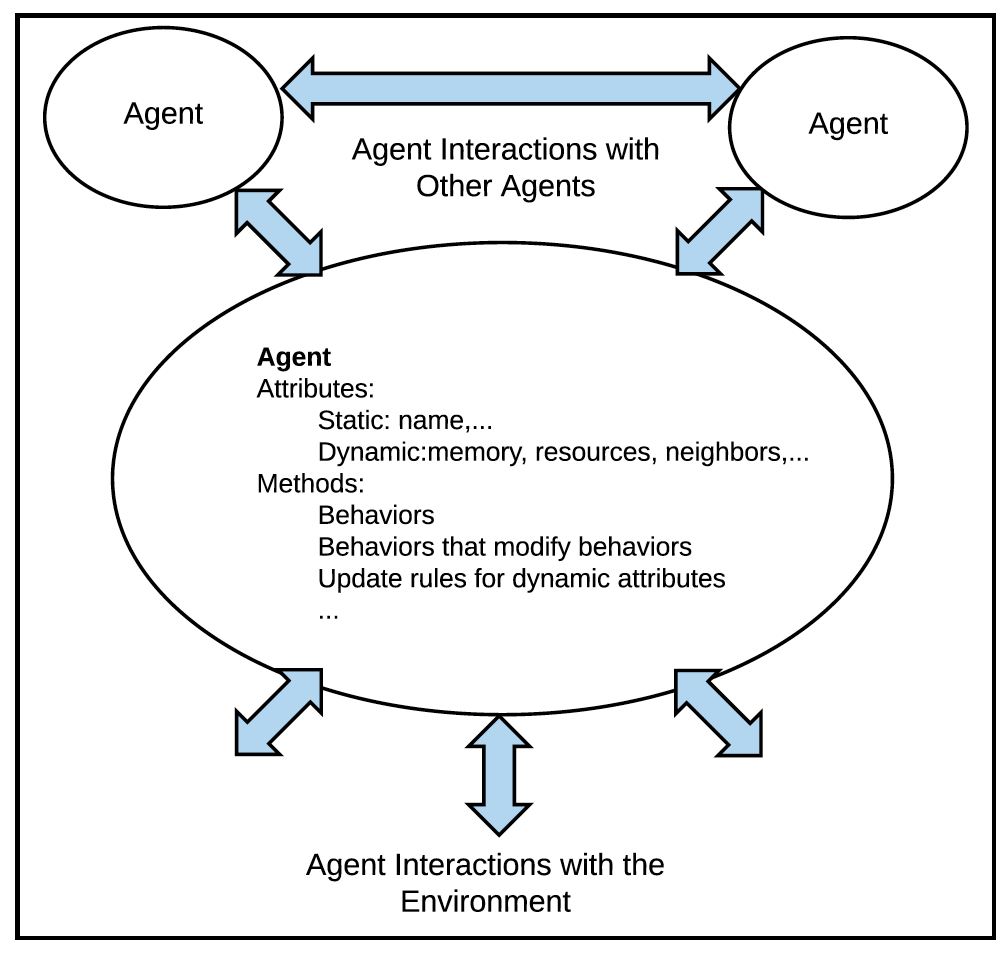
\includegraphics[scale = 0.35]{agent_interactions}
% 	\caption{A typical agent \cite{macal2014introductory}}
% 	\label{fig:agent_interactions}
% \end{figure}

\subsection{ABM for Disaster Management}
Agent-based modeling has numerous applications. In one study, agent based modeling was used to simulate crowd evacuation in case of a fire disaster in a concert venue \cite{wagner2014agent}. With the use of agent-based models, a prototype was developed to mimic a setting of a concert venue where the user can customize the parameter settings of the prototype’s environment. In another study, an ABM of flood incident management (FIM) was developed to provide new insights about flood management which could aid in policy analysis. The multi-agent simulation combined with a hydrodynamic model approximated individuals’ susceptibility to flooding. After testing the methods in a specific location, results showed that the model can be used to assess the effectiveness of flood management measures \cite{dawson2011agent}.
	
	In a similar manner, utilization of pedestrian lanes during crowd evacuation was modeled using agent-based modeling where the focus was on discovering which pedestrian lanes can be easily recognized during a disaster \cite{wu2012personalized}. Lanes which has a higher probability to be overcrowded and lanes that are less likely to be traversed by individuals during a disaster were identified using the collected data. The information gathered was used to make lanes visible and to distribute crowd traffic to those lanes thus preventing overcrowding in some lanes during evacuation.
	
	Anchoring on the UN’s cluster approach on information-processing, one study used agent-based modeling and simulation to demonstrate that properly used clusters promotes faster flow of information resulting in a timely and successful response to disasters \cite{altay2014information}. Findings showed that humanitarian response is immediately prompted if cluster leads will act as information hub and if information is shared eagerly. The study also showed that the higher the quality of information, the faster it moves, which is essential for effective resource utilization.
	
	ABM was also used in several studies that focused on human behavior during earthquake and tsunami. In one study, an evacuation model coupled with a numerical simulation of a tsunami and estimation evaluation of casualties was developed using Netlogo \cite{mas2012agent}. Performing simulations with 1,000 repetitions of evacuations using a specified location resulted in a very high mean of people evacuated. The simulation result tallied with the recorded evacuation and sheltered evacuee’s outcome after the actual event. Another study about earthquake evacuation behavior developed an agent-based behavioral model that describes phases and rules of motion for pedestrians during earthquake evacuation. Videotapes showing real events were used in conceptualizing the model \cite{d2014agent}. 

    
    Many studies have used agent-based modeling for different purposes. However, very little study has been gathered so far that used ABM to understand human behavior during disasters. This study will attempt to analyze disaster behavior using agent-based modeling.
    
\section{Household Evacuation Behavior during Typhoon and Flooding}
Typhoon causes several hazards like strong winds, flooding and landslides due to incessant rain and storm surge prompting at-risk households to evacuate to safe places. Most evacuations during typhoons are conducted in areas that are prone to flooding. Household’s decision to evacuate, however, is not only based on a single factor but on several ones according to several studies \cite{lim2016household, medina2016should, fu2004sequential, fu2006sequential, cahyanto2014empirical, stopher2004dynamic, fu2004sequential, whitehead2000heading}. As found out by various studies, the significant factors that influences the decision to evacuate are the characteristics of the decision-maker in the household, capacity-related factors and hazard-related factors \cite{lim2016household}. 

Identified decision maker’s attributes includes gender \cite{whitehead2000heading, cahyanto2014empirical, lim2016household}, age \cite{whitehead2000heading, cahyanto2014empirical, lim2016household}, level of education \cite{whitehead2000heading, hasan2010behavioral, lim2016household, medina2016should}, presence of young children \cite{whitehead2000heading, cahyanto2014empirical, lim2016household, medina2016should}, presence of elderly \cite{whitehead2000heading, cahyanto2014empirical}, presence of pet \cite{whitehead2000heading},  income level \cite{whitehead2000heading, cahyanto2014empirical, medina2016should}, house ownership \cite{lim2016household, hasan2010behavioral}, length of stay in residence \cite{lim2016household} and number of household members \cite{cahyanto2014empirical}. Housing type and previous typhoon experience on one hand are classified as capacity-related factors \cite{whitehead2000heading, fu2004sequential, fu2006sequential, hasan2010behavioral}. Finally, there are hazard-related factors that affects evacuation decision: distance to typhoon \cite{fu2004sequential, fu2006sequential}, typhoon forward speed \cite{fu2004sequential, fu2006sequential}, typhoon wind speed \cite{fu2006sequential}, presence of evacuation message \cite{fu2006sequential, hasan2010behavioral}, possibility of flooding \cite{fu2004sequential, fu2006sequential, hasan2010behavioral}, time of the day \cite{fu2004sequential, fu2006sequential}, source of notice for evacuation \cite{hasan2010behavioral} and type of evacuation notice received \cite{hasan2010behavioral}. 

In a household-level evacuation decision model done by one study \cite{lim2016household} for a large city in the Philippines, their model estimation for partial and full evacuation gave the following results: compared to a female household head, there is a higher probability of not evacuating the members of the household if the head is male which is in consonance with the findings of other studies \cite{horney2010individual, lindell2005household, morrow2005hurricane}; there is a higher probability that the households living in a house with more than 1 floor level will not evacuate; there is less likelihood that households will not evacuate if the level of house damage is high; households who own the house are more likely to evacuate compared to those who are just renting; households with homes made from concrete materials have a higher probability of staying at home compared to households whose houses are made of wood; if the source of evacuation warning came from the authorities then the households are more likely to evacuate compared to when the source of information came from relatives or friends; in the presence of small children, households are likely to evacuate which supports the results of other studies \cite{cahyanto2014empirical, fischer1995evacuation, dash2002decision}; and households that are located more than 10 meters away from the source of flood hazard have a high probability of evacuating. These results are used as reference by this study for formulating decision model for human behavior during typhoon evacuation. Moreover, results of other studies \cite{medina2016should, fu2004sequential, fu2006sequential, cahyanto2014empirical, stopher2004dynamic, fu2004sequential, whitehead2000heading} on evacuation behavior were also considered.

% ++++++++++++++++++++++++++++++++++++++++++++++++++++++++

\section{Public Storm Warning System and Rainfall Warnings in the Philippines}
The Philippines' weather state bureau Philippine Atmospheric, Geophysical and Astronomical Services Administration (PAGASA) uses its Public Storm Warning System to categorize typhoon intensity and warn the public. The Public Storm Warning System has five Public Storm Warning Signals (PSWS). The purpose of hoisting a storm signal number over a locality is to warn the public about the impending typhoon. PSWS \#1 is 

When any Public Storm Warning Signal Number is hoisted or put in effect for the first time, the corresponding meteorological conditions are not yet prevailing over the locality. This is because the purpose of the signal is to warn the impending occurrence of the given meteorological conditions. It must be noted also that the approximate lead time to expect the range of the wind speeds given for each signal number is valid only when the signal number is put in effect for the first time. Thus, the associated meteorological conditions are still expected in at least 36 hours when PSWS \#1 is put in effect initially; in at least 24 hours with PSWS \#2; in at least 18 hours with PSWS \#3, in at least 12 hours with PSWS \#4; and in at least 12 hours with PSWS \#5. The lead time shortens correspondingly in the subsequent issues of the warning bulletin when the signal number remains in effect as the tropical cyclone comes closer.


It is also important to remember that tropical cyclones are constantly in motion; generally towards the Philippines when PAGASA is issuing the warning. Therefore, the Public Storm Warning Signal Number over a threatened/ affected locality may be sequentially upgraded or downgraded. This means that PSWS \#1 may be be upgraded to PSWS \#2, then to PSWS \#3, PSWS \#4 and to PSWS \#5 as necessary when a very intense typhoon is approaching or downgraded when the typhoon is moving away. However, in case of rapid improvement of the weather condition due to the considerable weakening or acceleration of speed of movement of the tropical cyclone moving away from the country, the downgrading of signal may jump one signal level. For example, PSWS \#3 may be downgraded to PSWS \#1 or all signals from PSWS \#2 may be lowered.

The delineation of areas for a given signal number is based on the intensity, size of circulation and the forecast direction and speed of movement of the tropical storm or typhoon at the time of issue of the warning bulletin. The change in intensity, size of circulation or movement of the tropical cyclone also determines the change in the PSWS number over a given locality.


Every year, around 20 tropical cyclones visit the country, making flood a perennial problem for Filipinos.

\begin{table}[!htbp]
\centering
\caption{Public Storm Warning System}
% Also use the label tag
\label{Table:PSWS}
\begin{tabular}{|p{1.2cm}|p{1.3cm}|p{1.4cm}|p{5.1cm}|}
\hline
% \textbf{PSWS} & \textbf{Lead Time (hrs)} & \textbf{Winds (kph)} & \textbf{Impacts of the Wind} \\
PSWS & Lead Time (hrs) & Winds (kph) & Impacts of the Wind \\\hline
\#1 & 36 & 30 - 60 & No damage to very light damage \\
\#2 & 24	& 61 - 120 & Light to moderate damage	\\                                      
\#3 & 18 & 121 - 170 & Moderate to heavy damage \\
\#4 & 12 & 171 - 220 & Heavy to very heavy damage \\
\#5 & 12 & $>$ 220 & Very heavy to widespread damage \\
\hline
\end{tabular}
\end{table}



% \begin{table}[!htbp]
% \centering
% \caption{Color-Coded Rainfall Advisories}
% % Also use the label tag
% \label{Table:PSWS}
% \begin{tabular}{p{0.7cm}p{2.5cm}p{3.5cm}}
% \hline
% \textbf{Levels} & \textbf{Rain Measurement} & \textbf{Meaning} \\ \hline
% Yellow & 7.5 - 15 mm rain. \qquad Observed in 1 hour and expected to continue in the next 2 hours.  & $<$Community Awareness$>$. Flooding is possible in low lying areas and near river channels. \\
% Orange & 15 - 30 mm rain. \qquad Observed in 1 hour and expected to continue in the next 2 hours. & $<$Community Preparedness$>$. Flooding is threatening in low-lying areas and near river channels.	\\                                      
% Red & More than 30mm rain. Observed in 1 hour and expected to continue in the next 2 hours. & $<$Community Response$>$. \qquad Severe flooding is expected. Take necessary precautionary measures. \\
% \hline
% \end{tabular}
% \end{table}

\begin{table}[htbp]
\centering
\caption{Color-Coded Rainfall Advisories.}\label{tab1}
%\label{Table:PSWS}
%\begin{tabular}{|l|l|l|}
\begin{tabular}{|p{1.5cm}|p{5cm}|p{5cm}|}
\hline
Levels &  Rain Measurement & Meaning\\
\hline
Yellow &  7.5 - 15 mm rain. Observed in 1 hour and expected to continue in the next 2 hours. & $($Community Awareness$)$. Flooding is possible in low lying areas and near river channels.\\
Orange &  15 - 30 mm rain. Observed in 1 hour and expected to continue in the next 2 hours. & $($Community Preparedness$)$. Flooding is threatening in low-lying areas and near river channels.\\
Red & More than 30mm rain. Observed in 1 hour and expected to continue in the next 2 hours. & $($Community Response$)$. Severe flooding is expected. Take necessary precautionary measures.\\
\hline
\end{tabular}
\end{table}


In 2012, Philippines' state weather bureau PAGASA released a set of color-coded rainfall advisories which is composed of 3 colors: Yellow, Orange and Red. Yellow advisory means heavy rainfall of 7.5 - 15 mm in an hour is observed and is expected to continue for the next 2 hours. This can be equivalent to 2 gallons of rain per square meter per hour. When this advisory is given by PAGASA, it means that residents in affected areas should continue monitoring their weather condition. Flooding for low-lying areas is possible. Orange advisory on the other hand means intense rainfall of 15-30mm in an hour is observed and is expected to continue for the next 2 hours. This can be equivalent to 4 to 8 gallons of rain per square meter per hour. When PAGASA gives Orange advisory, it means that residents in affected areas should be on alert for possible evacuation. Flooding in affected areas is expected. Finally, a Red advisory means torrential rainfall of more than 30mm in an hour is observed and is expected to continue for the next 2 hours. This can be equivalent to 8 gallons of rain per square meter per hour. When PAGASA gives Red advisory, it means that severe flooding in low lying areas is expected and residents should take the necessary precautionary measures.

% source: http://bagong.pagasa.dost.gov.ph/learning-tools/public-storm-warning-signal
% source: https://www1.pagasa.dost.gov.ph/index.php/20-weather/29-rainfall-warnings


\section{Methodology}     

\subsection{Model Overview}
\subsubsection{Purpose of the Model}
The purpose of the model is to initially understand human behavior during disaster event such as typhoon. It is designed particularly for decision makers who are engaged in disaster risk reduction and management. 

\subsubsection{Entities, State Variables and Scales}
There are three types of human agents in the model. These are households, rescuers, and shelter managers. The household agents are characterized by the attributes of the head of the household: location, gender, income level, level of education, has small kids in the household, has elderly in the household, has household member with physical disability, type of house ownership, years of residency, past typhoon experience, and perceived risk. Rescuer agents are characterized by their location, vitality, proximity from the source of hazard, and perceived risk. On the other hand, a Shelter Manager agent is characterized by the capacity of the evacuation shelter it is assigned to. 

Typhoon wind intensity and rainfall severity are the exogenous factors/drivers of the model. The space in the model is a georeferenced GIS data. Each household agent is assigned to a building(house) and each evacuation center has an assigned shelter manager agent. Rescuer agents are traced through their location coordinates. 

Each time step in the model represents BLANK. The temporal extent of the model is BLANK time steps (8 hrs?). The spatial resolution is not relevant in this model. The spatial extent of the model is one village or ‘barangay’.

\subsubsection{Process Overview and Scheduling}
The model has two phases, the set up (initialization) phase and the run (simulation) phase. Initialization is initiated when time-step = 0. During this phase, values are initialized or assigned to identity variables of each type of agents. Parameters of the model are also initialized during this time. 

The run or simulation phase is carried on for each time step from 1 to 8. If time-step = 8, then the simulation halts. The model situation at the start of the simulation is when the typhoon is hours away before hitting land. Before the typhoon hits the village, rescuer agents roams around the village and informs the household agents about the impending typhoon, then announces preemptive evacuation.  During this time, household agents computes their perceived risk. If the computed perceived risk is higher than the VALUE then the household agent evacuates to the nearest evacuation shelter inside the village or outside of it. However, if the perceived risk value is lower than the VALUE, then the household agent stays (does not evacuate). Shelter Manager agents accepts evacuees in evacuation centers and keeps check on the shelter’s maximum capacity. If maximum capacity of the shelter is reached then incoming evacuees will be directed to other evacuation shelters.
% 3.	During landfall of the typhoon:
% ♣	Rescuers monitors for possible household agents that might ask for help. However, if the computed perceived risk value of the rescuer agent reaches dangerous values , it will cease its rescue operation. 

\subsection{Design Concepts}
\subsubsection{Theoretical and Empirical Background}
1.1.1.	Which general concepts, theories or hypotheses are underlying the model’s design at the system level or at the level(s) of the sub model(s) (apart from the decision model)? What is the link to the complexity and the purpose of the model?

(To Do)
1.1.2.	On what assumptions is/are the agents’ decision model(s) based?

(To Do)

1.1.3.	Why is/are certain decision model(s) chosen?

(To Do)

1.1.4.	If the model/sub-model (e.g. the decision model) is based on empirical data, where do the data come from?

The empirical data come from several sources:
o	The survey and results of several studies about evacuation during typhoon and flooding.
o	Census and housing data from the Philippine Statistics Agency and local (Municipal) census data as well as disaster report from Municipal Disaster Risk Reduction and Management Office (MDRRMO).  

The level of aggregation is available at the household level.

\subsubsection{Individual Decision-Making}
1.1.1.	What are the subjects and objects of decision-making? On which level of aggregation is decision-making modelled? Are multiple levels of decision making included?

The subjects of decision-making are household agents, rescuer agents, and shelter manager agents. The decision-making is observed at the level of household agents, rescuer agents, and shelter manager agents. The objects of decision making for household agents are: characteristics  of the head of household or decision maker; capacity-related factors; hazard-related factors; and presence of a household neighbor asking for help. The objects of decision making for rescuer agents are household agents at-risk, presence of hazards, and their vitality status (value). The object of decision making for shelter manager agent is the capacity of the evacuation shelter it is assigned to.  

1.1.1.	What is the basic rationality behind agent decision-making in the model?

The household agents’ main aim is to survive the onslaught of typhoon. The rescuer agents aim is to achieve zero casualty by informing household agents about the typhoon in advance, announcing preemptive evacuation and rescuing household agents at risk if possible. Shelter manager agents manages order and capacity of the evacuation center.

1.1.1.	Do agents pursue an explicit objective or have other success criteria?

No, all agents makes decisions based on their decision heuristics and they do not follow an explicit objective.

1.1.1.	How do agents make their decisions?
Household agents computes their perceived risk value in order to make a decision. The perceived risk depends on three decision factors: characteristics of decision maker; capacity-related factor; and hazard-related factor. Bounded rationality is incorporated in the perceived-risk equation by adding a random value from a known range of values.

Rescuer agents and shelter manager agents use decision trees when making a decision. For example, a rescuer agent will rescue a household agent that is nearest to it or the most at risk (the one with the highest perceived risk value among household agents asking for help). If two or more household agents have the same perceived risk value, then the one nearest to the source of hazard will be rescued first. In the case of shelter manager agent, it accepts evacuees only if the maximum capacity of the evacuation center is not exceeded. 

1.1.1.	Do the agents adapt their behavior to changing endogenous and exogenous state variables? And if yes, how?

Household and rescuer agents adapt to exogenous state variables since these variables have direct effect on their risk perception and individual objectives. For instance, an increasing public storm warning signal also increases the hazard-related factor value which is a component of the perceived risk equation for household agents. It also decreases the vitality of the rescuers as they perform rescue operations. In addition, changing decision states (from staying to evacuating) of household agents affects the behavior of neighboring agents, may it be other household agents or rescuer agents. A household agent might evacuate because the majority of its household agent neighbors evacuated already.  

Shelter managers, on the other hand, do not adapt their behavior from exogenous state variables. 

1.1.1.	Do social norms or cultural values play a role in the decision-making process?

Yes. The decision of other household agents to evacuate influence the evacuation decision of their neighboring household agents. 

1.1.1.	Do spatial aspects play a role in the decision process?

Yes. Since the model environment is a GIS data, the distance between objects is based from the real world. An agent that is near the source of hazard such as river will have a higher risk perception compared to others who are at a distance. Evacuating household agents also will choose the nearest available evacuation center. Moreover, a rescuer agent will prioritize the nearest at-risk household agent.

1.1.1.	Do temporal aspects play a role in the decision process?

Yes. Household agents perceives night time as a more risky situation compared to daytime during typhoon.

1.1.1.	To which extent and how is uncertainty included in the agents’ decision rules?

Uncertainty is not included in agents’ decision rules.

1.1.	Learning

1.1.1.	Is individual learning included in the decision process? How do individuals change their decision rules over time as a consequence of their experience?


1.1.2.	Is collective learning implemented in the model?

No.

\subsubsection{Individual Sensing}
1.1.1.	What endogenous and exogenous state variables are individuals assumed to sense and consider in their decisions? Is the sensing process erroneous?

Household agents and rescuer agents both sense the typhoon intensity and rainfall severity. Additionally, household agents can sense their individual risk perception while rescuer agents can perceive their vitality status.  
 
1.1.2.	What state variables of which other individuals can an individual perceive? Is the sensing process erroneous?

A household agent can sense the evacuation decisions of other household agents that are inside its perception area. Rescuer agents, on one hand, can sense household agents that are inside their perception area and those household agents who are asking for help.

1.1.3.	What is the spatial scale of sensing?

An agent can be sensed by another agent if it is inside the perception area (which is in a form a circle) of the former.

1.1.1.	Are the mechanisms by which agents obtain information modelled explicitly, or are individuals simply assumed to know these variables?

Individuals are assumed to know the variables.

1.1.2.	Are the costs for cognition and the costs for gathering information explicitly, or are individuals simply assumed to know these variables?

No.

The agents in this model has no prediction component.

\subsubsection{Interaction}
1.1.1.	Are interactions among agents and entities assumed as direct or indirect?

The interaction between household agents and rescuer agents, household agents and shelter managers and between household agents is direct.

1.1.2.	On what do the interactions depend?

Interactions depend on spatial distances. Each agent type has a perception area in a form of a circle based from perception radius. The perception radius of the agent is the distance where it can sense other agents. Household agents that are enclosed within a perception area is considered a neighborhood. A household agent could belong to several neighborhoods.

Interaction is assumed when one agent (household) asks for help or senses the evacuation decision of neighboring agents. 

1.1.3.	If the interactions involve communication, how are such communications represented?


1.1.4.	If a coordination network exists, how does it affect the agent behavior? Is the structure of the network imposed or emergent?

Not Applicable.

1.1.1.	Do the individuals form or belong to aggregations that affect and are affected by the individuals? Are these aggregations imposed by the modeler or do they emerge during the simulation?

No.
1.1.2.	How are collectives represented?

Not applicable.

\subsubsection{Heterogeneity}
1.1.1.	Are the agents heterogeneous? If yes, which state variables and/or processes differ between the agents?

The household agents are heterogeneous based on the attributes of the decision maker or head of household (gender, age, level of education, presence of elderly, presence of young children, income level, house ownership, length of stay in the residence, previous typhoon experience, housing type), their evacuation decision, awareness about other agents, and cooperation decision (cooperate or defect).

Rescuer agents on the other hand are heterogeneous based on their vitality and mechanism on carrying rescue operations.
 
1.1.2.	Are the agents heterogeneous in their decision-making? If yes, which decision models or decision objects differ between the agents.

\subsubsection{Stochasticity}
1.1.1.	What processes (including initialization) are modelled by assuming they are random or partly random?

The initial positions of household agents and rescuer agents is randomized. Although houses and buildings in the model environment are fixed, heterogeneous household agents are randomly assigned to each of them. The order in which household agents decides to evacuate is also random as it depends on their individual perceived risk value. The direction in which the rescuers are headed to inform households about preemptive evacuation is also random. 

\section{Implementation Details}
1.1.	Implementation Details

1.1.1.	How has the model been implemented?

The model is implemented using GAMA Platform V1.8.0

\subsubsection{Initialization}
1.1.1.	What is the initial state of the model world, i.e. at time t=0 of a simulation run?

At time t = 0, there are 570 household agents that are initialized and randomly assigned to houses/buildings. There are also 15 to 21 rescuer agents randomly placed to their initial positions and 4 shelter managers assigned to four evacuation centers inside the barangay. 

…More here about the initial weights of decision factors.

1.1.2.	Is the initialization always the same, or is it allowed to vary among simulations?

The initialization for household agents is always the same but the initial values for rescuers and shelter managers can be varied. 

1.1.3.	Are the initial values chosen arbitrarily or based on data?

The initial values are based on data. These data are sourced from census data and interviews.

\subsubsection{Input Data}

1.1.1.	Does the model use input from external sources such as data files or other models to represent processes that change over time?

No.

\subsubsection{Sub-models}

1.2.1.	What, in detail, are the sub-models that represent the processes listed in ‘Process overview and scheduling’?

1.1.1.	What are the model parameters, their dimensions and reference values?

Household Agent’s State Variables


1.1.1.	How were the sub-models designed or chosen, and how were they parameterized and then tested?
(ToDo)



% ++++++++++++++++++++++++++++++++++++++++++++++++++++++++
\subsection{Conceptual Model}

\begin{figure}[!ht]
    \centering
    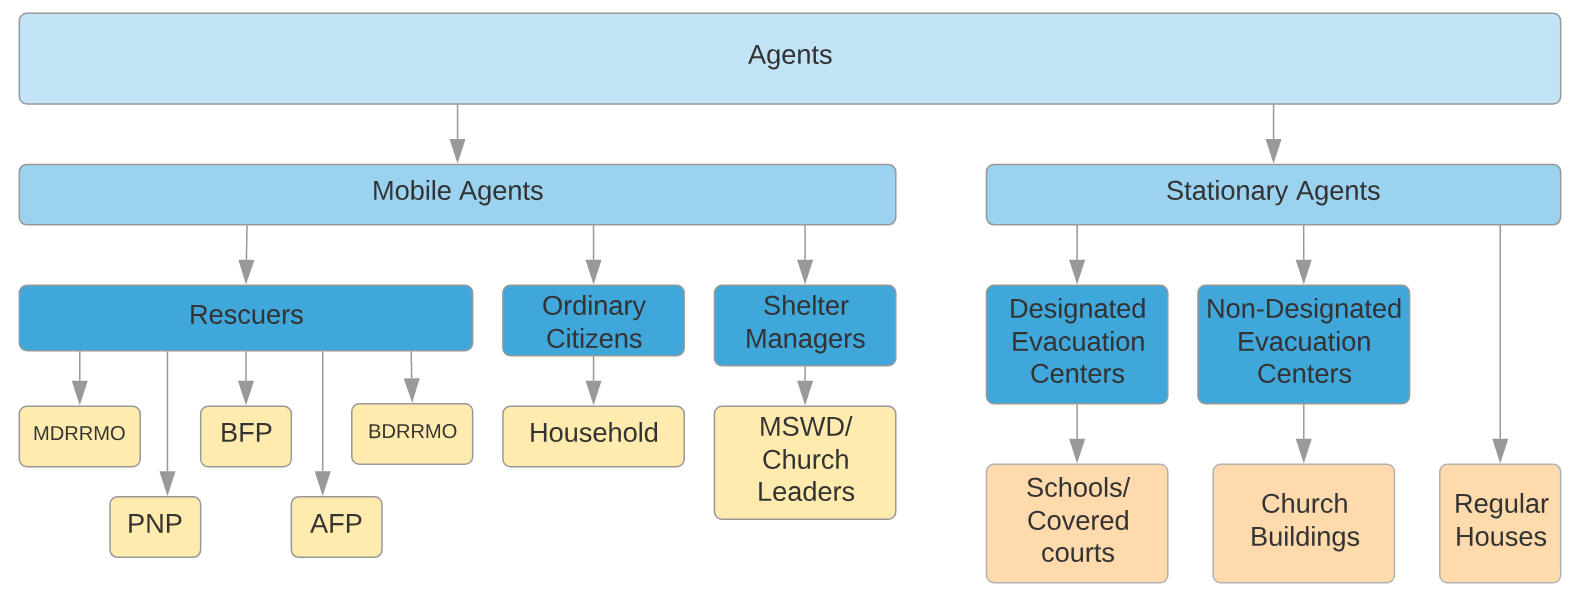
\includegraphics[scale = 0.30]{_abms_agents.png}
	\caption{Type of Agents in the Model}
	\label{fig:agent_types}
\end{figure}

The agents in this agent-based model are of two types: mobile agents and stationary agents. Mobile agents refers to human agents that are involved during disaster response and rescue operations which includes the rescuers, shelter managers and ordinary citizens. Stationary agents on the other hand are considered part of the environment of agents. Stationary agents includes designated and non-designated evacuation centers or shelters as well as regular buildings and houses. These structures have attributes that mobile agents monitors for decision making. Figure \ref{fig:agent_types} shows the different agents for the proposed ABM. 

\begin{figure}
\centering
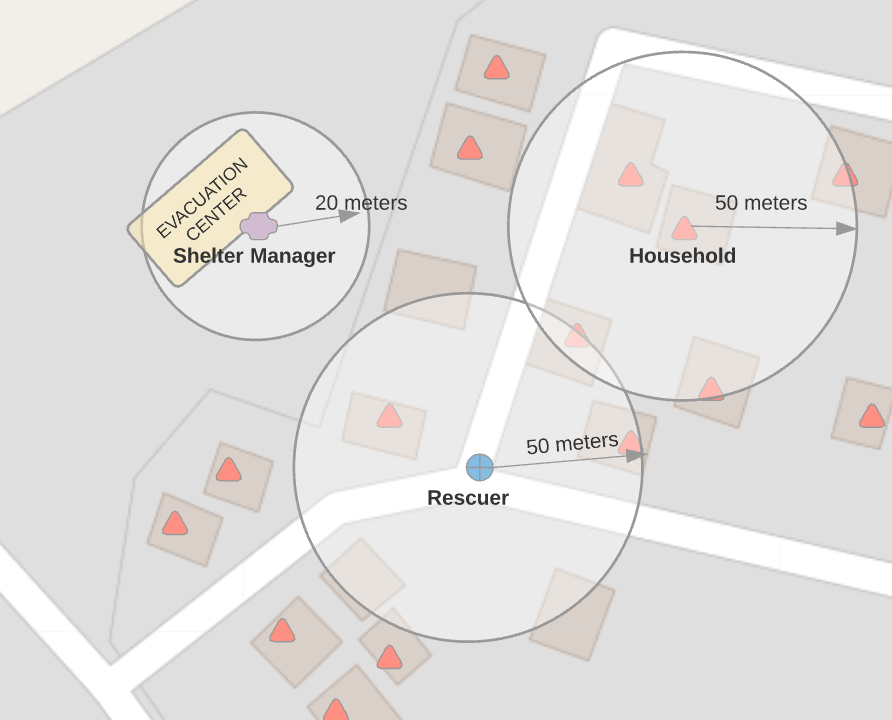
\includegraphics[scale=0.6]{_perception_distances.png}
\caption{Perception Distances of Household, Rescuer and Shelter Manager Agents.} \label{_perception_distances}
\end{figure}

\begin{figure}
\centering
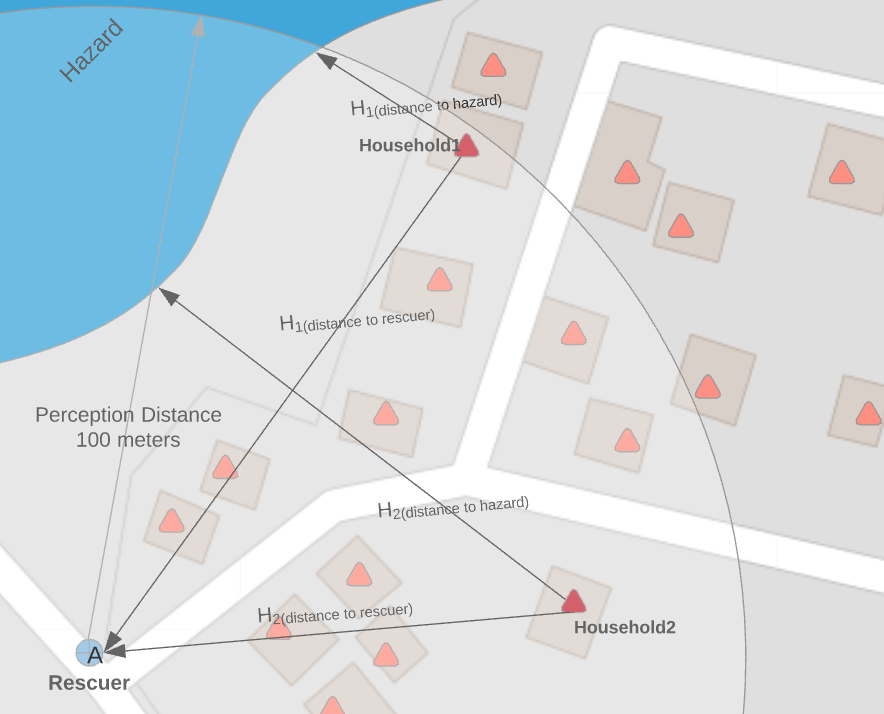
\includegraphics[scale=0.6]{_priority_distance.png}
\caption{A figure caption is always placed below the illustration. Please note that short captions are centered, while long ones are justified by the macro package automatically.} \label{_abms_distance_priority}
\end{figure}

\begin{figure}
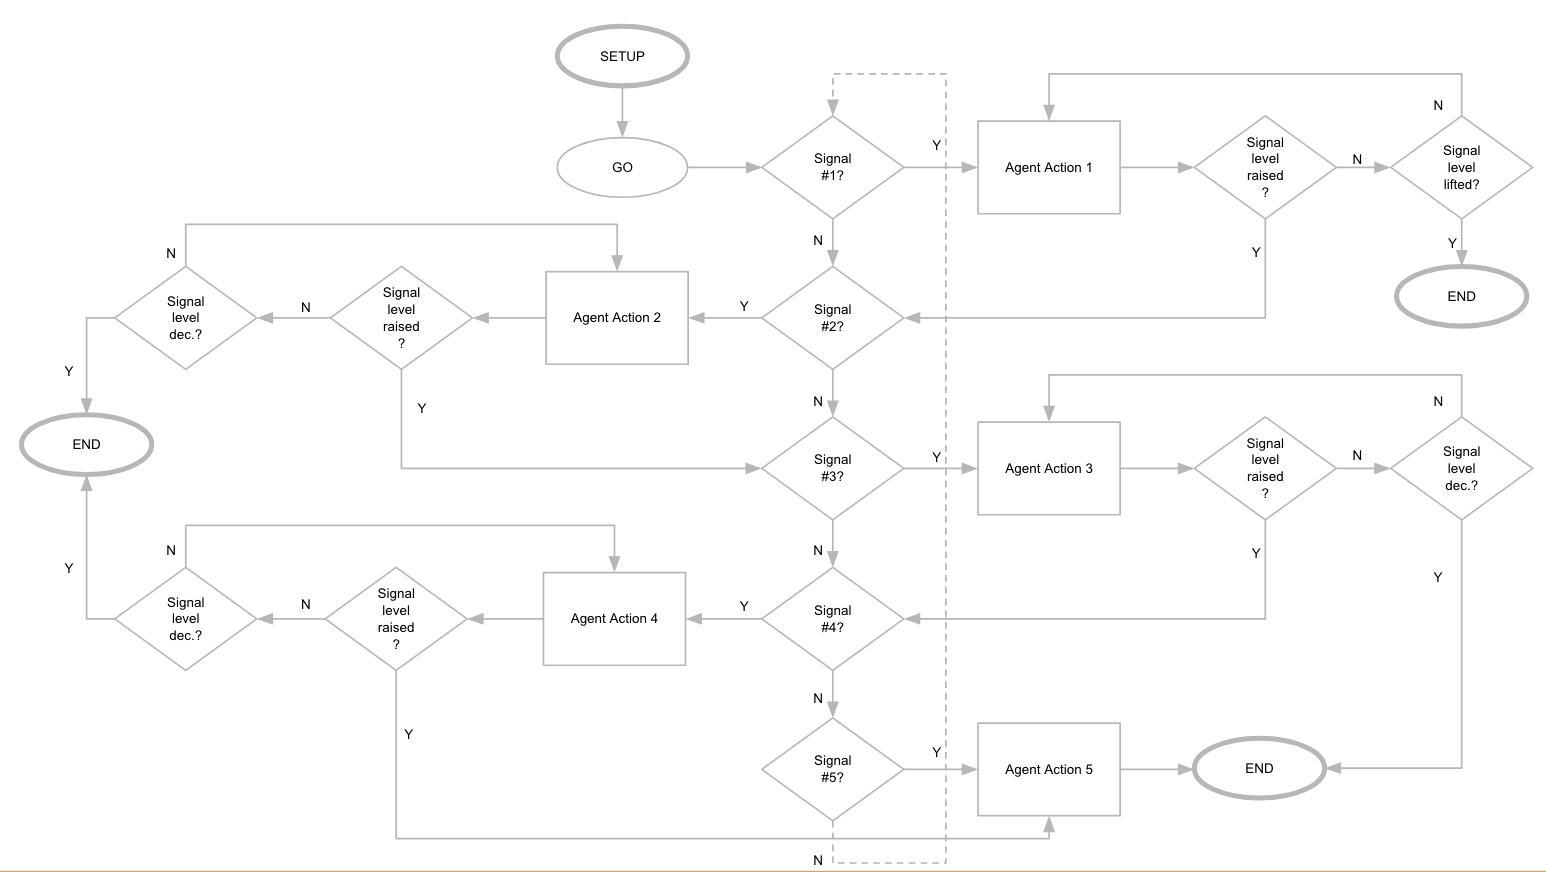
\includegraphics[width=\textwidth]{_abms_gendiagram_oc.png}
\caption{A figure caption is always placed below the illustration. Please note that short captions are centered, while long ones are justified by the macro package automatically.} \label{abms_gendiagram_oc}
\end{figure}

\begin{figure}
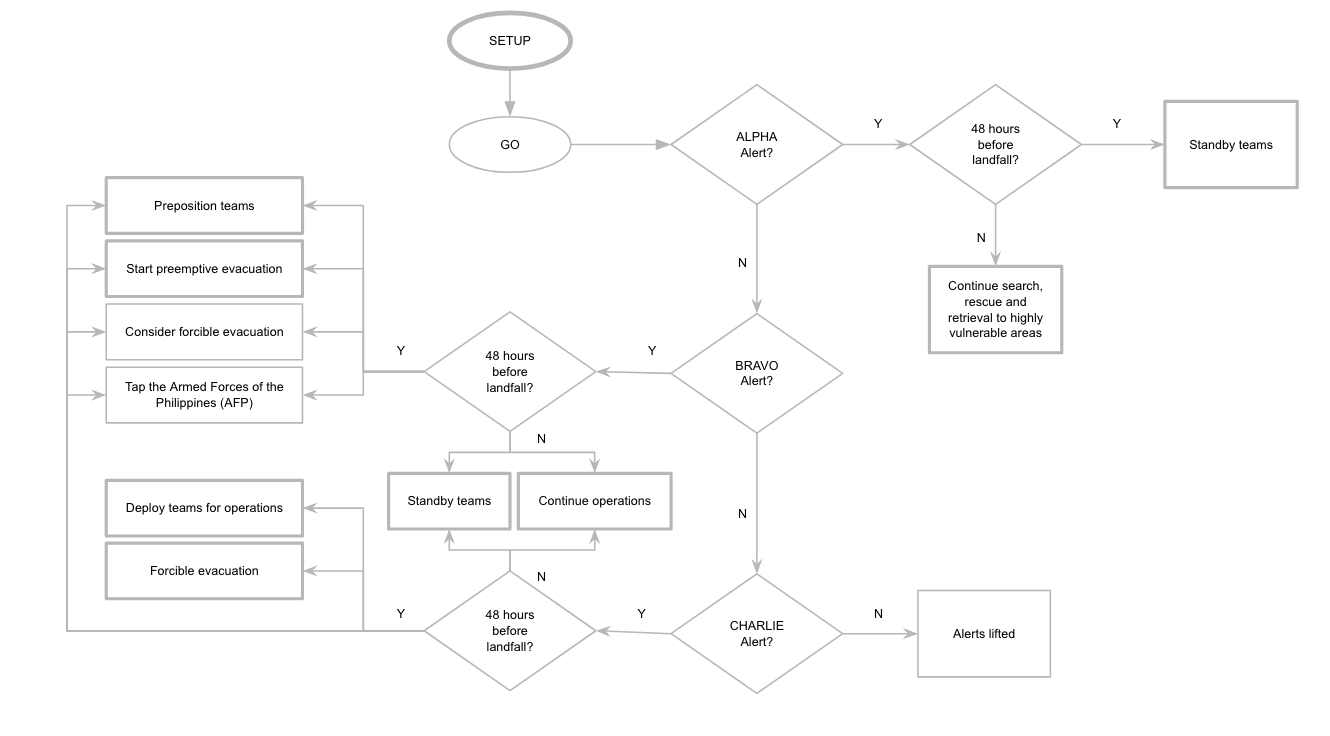
\includegraphics[width=\textwidth]{_abms_gendiagram_rr.png}
\caption{A figure caption is always placed below the illustration. Please note that short captions are centered, while long ones are justified by the macro package automatically.} \label{abms_gendiagram_rr}
\end{figure}

\begin{figure}
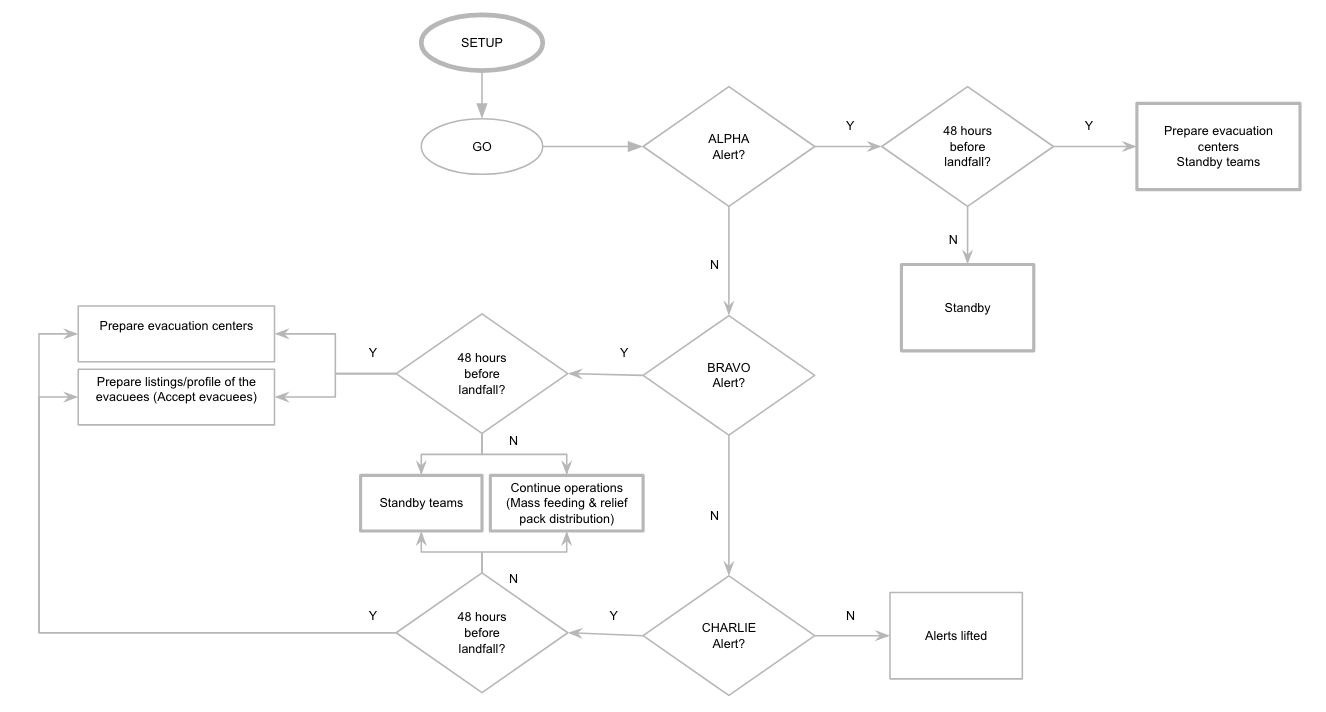
\includegraphics[width=\textwidth]{_abms_gendiagram_sm.png}
\caption{A figure caption is always placed below the illustration. Please note that short captions are centered, while long ones are justified by the macro package automatically.} \label{abms_gendiagram_sm}
\end{figure}

\begin{figure*}[!ht]
    \centering
    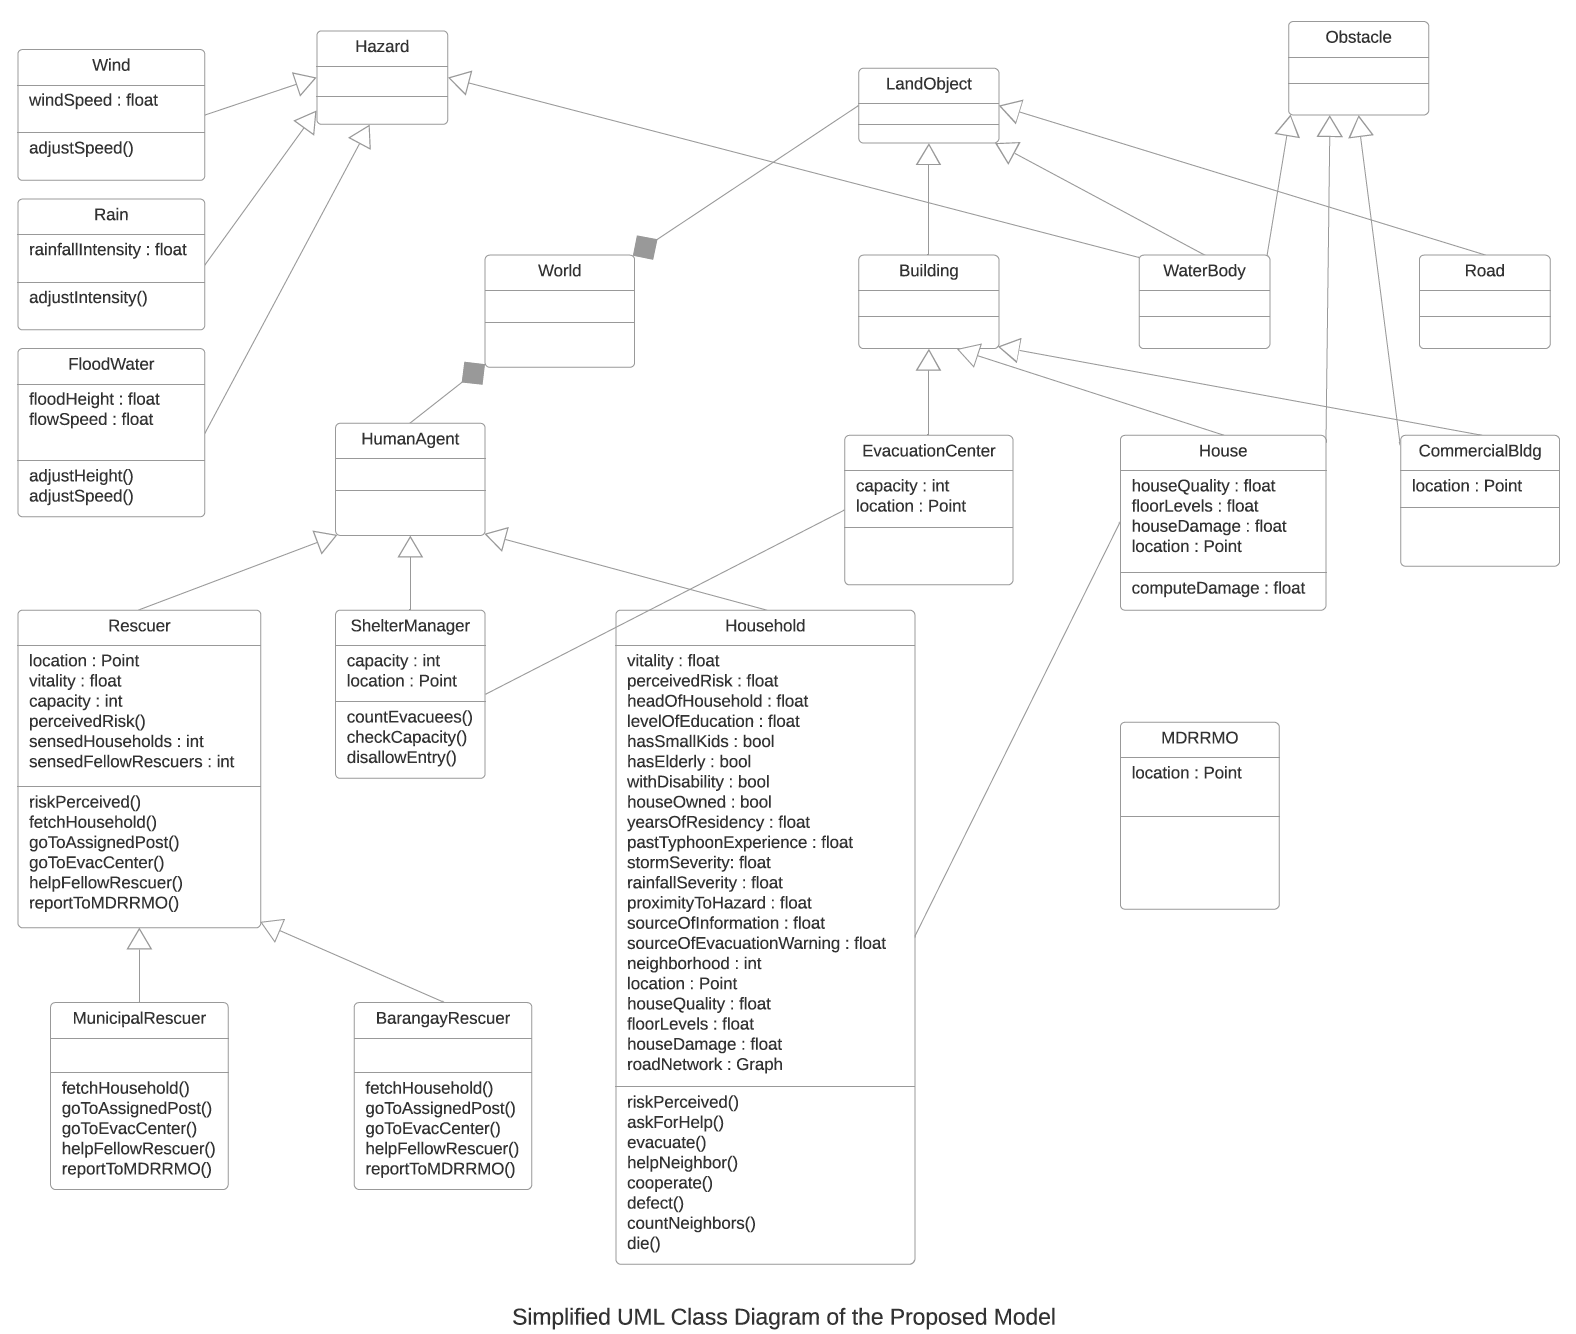
\includegraphics[width=\textwidth,height=10cm]{uml-abm.png}
	\caption{Simplified UML Diagram of the Model}
	\label{fig:simplified_uml}
\end{figure*}


\begin{table*}[htb]
\begin{center}
\caption{Characteristics of Decision Maker and Corresponding Values}
{\small
\hfill{}
\begin{tabular}{|p{5cm}|p{1.5cm}|p{1cm}|p{1.5cm}|p{1cm}|p{1.5cm}|p{1cm}|}
\hline
Characteristics of Decision Maker & & Value & & Value & & Value \\
\hline
gender & male & 0.5 & female & 1.0 & & \\
level of education & college & 0.4 & high school & 0.7 & elementary & 1.0 \\
presence of young children & no & 0 & yes & 1 & & \\
presence of elderly & no & 0 & yes & 1 & & \\
presence of household member with disability & no & 0 & yes & 1 & & \\
income level & high & 0.4 & medium & 0.7 & low & 1.0 \\
house ownership & no & 0 & yes & 1 & & \\
length of stay in residence & $>$ 10 years & 0.5 & $\geq$ 10 years & 1.0 & & \\
\hline
\end{tabular}}
\hfill{}
%\caption{Table Name}
\label{keynodes_a}
\end{center}
\end{table*}

\begin{table*}[htb]
\begin{center}
\caption{Capacity-Related Factors and Corresponding Values}
{\small
\hfill{}
\begin{tabular}{|p{4cm}|p{1.5cm}|p{1cm}|p{1.5cm}|p{1cm}|p{2cm}|p{1cm}|}
\hline
Capacity-Related Factor & & Value & & Value & & Value \\
\hline
house quality & concrete & 0.4 & wood & 0.7 & light materials & 1.0 \\
house floor levels & $>$1 level & 0.5 & 1 level & 1.0 &  &  \\
past typhoon experience & yes & 0.5 & no & 1.0 & & \\
\hline
\end{tabular}}
\hfill{}
%\caption{Table Name}
\label{keynodes_a}
\end{center}
\end{table*}

\begin{table*}[htb]
\begin{center}
\caption{Hazard-Related Factors and Corresponding Values}
{\small
\hfill{}
\begin{tabular}{|p{4.5cm}|p{1.5cm}|p{1cm}|p{1.5cm}|p{1cm}|p{2cm}|p{1cm}|}
\hline
Hazard-Related Factor & & Value & & Value & & Value \\
\hline
storm severity & PSWS \#1 & 0.4 & PSWS \#2 & 0.7 & PSWS \#3-5 & 1.0 \\
rainfall severity & yellow & 0.4 & orange & 0.4 & red & 1.0 \\
proximity to the source of hazard & far & 0.4 & near & 0.7 & within & 1.0 \\
source of evacuation warning & friends & 0.4 & media & 0.7 & authorities & 1.0 \\
time of day & daytime & 0.5 & night time & 1.0 & & \\
\hline
\end{tabular}}
\hfill{}
%\caption{Table Name}
\label{keynodes_a}
\end{center}
\end{table*}

\subsection{System Specification}

\subsection{Implementation of the Model}

\subsection{Agent-Based Modeling of Disaster Behavior}

\begin{equation} \label{eq:priorityHousehold}
	PriorityScore = \frac{1}{D_{hazard}^{p} * D_{rescuer}^{1-p}} 
\end{equation}

where $0 < p \leq 1$ and $increment \quad step = 0.1$

\begin{equation}\label{eq:perceivedRisk}
    \resizebox{0.95\hsize}{!}{%
	$PerceivedRisk = \sum\limits_{f=1}^{3}(DecisionFactorScore_{hf} * weight) + \varepsilon$%
	}
\end{equation}

where $\varepsilon$ is the bounded rationality with value 0.0 to 0.05.

\subsection{Tool used for Agent-Based Modeling}
There are several software that can be used for agent-based modeling... 

\subsection{Movement Rules}
In this model, movement rules govern the evacuation activities of all mobile agents. Each time step represents 10-minute interval for the duration of 54 hours. 
% $P_{exp}$ is the probability that a rescuer moves to the vulnerable areas and is arbitrarily set to 0.9. However, a stochastic perturbance value $P_{stoc}$ that is between 0 and 1 will be computed for each possible destination to model the non-linearity of human decision making. When $P_{stoc} > P_{exp}$, a destination option is randomly selected from areas near or within the hazard zones.

% ASSUMPTIONS
%- The probable destination for a rescuer are those areas in the hazard zones. 
%- A rescuer knows the location of evacuation centers in his designated areas. 
%- A rescuer could be any of the two: member of the strike team or member of BDRRMO.
% How do we set the neighborhood configuration for the NPPD game play?

\subsection{Interaction Neighborhoods}

As mentioned in one study \cite{power2009spatial}, the “depth of an interaction neighborhood defines the extents of the spatial association of a social grouping within the environment”. The neighborhood of an agent is determined based on the proximity of other agents to it. In this agent-based model, the neighbors of an agent are those nearby agents that fall inside the agent’s perception area. A perception area will be represented by a circle surrounding the agent. The distance from the agent to the circumference of the circle is its perception distance. For each time step, all agents that are within the perception distance of a certain agent, whether mobile or stationary, will be regarded as “seened” by that agent and will be saved in its memory. This agent perception or sensing ability also senses the environment terrain and the presence of hazards.  




% ++++++++++++++++++++++++++++++++++++++++++++++++++++++++

\section{Preliminary Results}
% ++++++++++++++++++++++++++++++++++++++++++++++++++++++++
% \subsection{ToDo}
1.1.	Observation

1.1.1.	What data are collected from the ABM for testing, understanding and analyzing it, and how and when are they collected?

To Be Determined.
1.1.2.	What key results, outputs or characteristics of the model are emerging from the individuals? (Emergence)

To Be Determined.


\section{Conclusion}






\subsection{A Subsection Sample}
Please note that the first paragraph of a section or subsection is
not indented. The first paragraph that follows a table, figure,
equation etc. does not need an indent, either.

Subsequent paragraphs, however, are indented.

\subsubsection{Sample Heading (Third Level)} Only two levels of
headings should be numbered. Lower level headings remain unnumbered;
they are formatted as run-in headings.

\paragraph{Sample Heading (Fourth Level)}
The contribution should contain no more than four levels of
headings. Table~\ref{tab1} gives a summary of all heading levels.

% \begin{table}
% \caption{Table captions should be placed above the
% tables.}\label{tab1}
% \begin{tabular}{|l|l|l|}
% \hline
% Heading level &  Example & Font size and style\\
% \hline
% Title (centered) &  {\Large\bfseries Lecture Notes} & 14 point, bold\\
% 1st-level heading &  {\large\bfseries 1 Introduction} & 12 point, bold\\
% 2nd-level heading & {\bfseries 2.1 Printing Area} & 10 point, bold\\
% 3rd-level heading & {\bfseries Run-in Heading in Bold.} Text follows & 10 point, bold\\
% 4th-level heading & {\itshape Lowest Level Heading.} Text follows & 10 point, italic\\
% \hline
% \end{tabular}
% \end{table}


% \begin{table}
% \caption{Table captions should be placed above the
% tables.}\label{tab1}
% \begin{tabular}{|l|l|l|}
% \hline
% Heading level &  Example & Font size and style\\
% \hline
% Title (centered) &  {\Large\bfseries Lecture Notes} & 14 point, bold\\
% 1st-level heading &  {\large\bfseries 1 Introduction} & 12 point, bold\\
% 2nd-level heading & {\bfseries 2.1 Printing Area} & 10 point, bold\\
% 3rd-level heading & {\bfseries Run-in Heading in Bold.} Text follows & 10 point, bold\\
% 4th-level heading & {\itshape Lowest Level Heading.} Text follows & 10 point, italic\\
% \hline
% \end{tabular}
% \end{table}


% \noindent Displayed equations are centered and set on a separate
% line.
% \begin{equation}
% x + y = z
% \end{equation}

% \begin{equation}
% x + y = z
% \end{equation}


Please try to avoid rasterized images for line-art diagrams and
schemas. Whenever possible, use vector graphics instead (see
Fig.~\ref{fig1}).

\begin{figure}
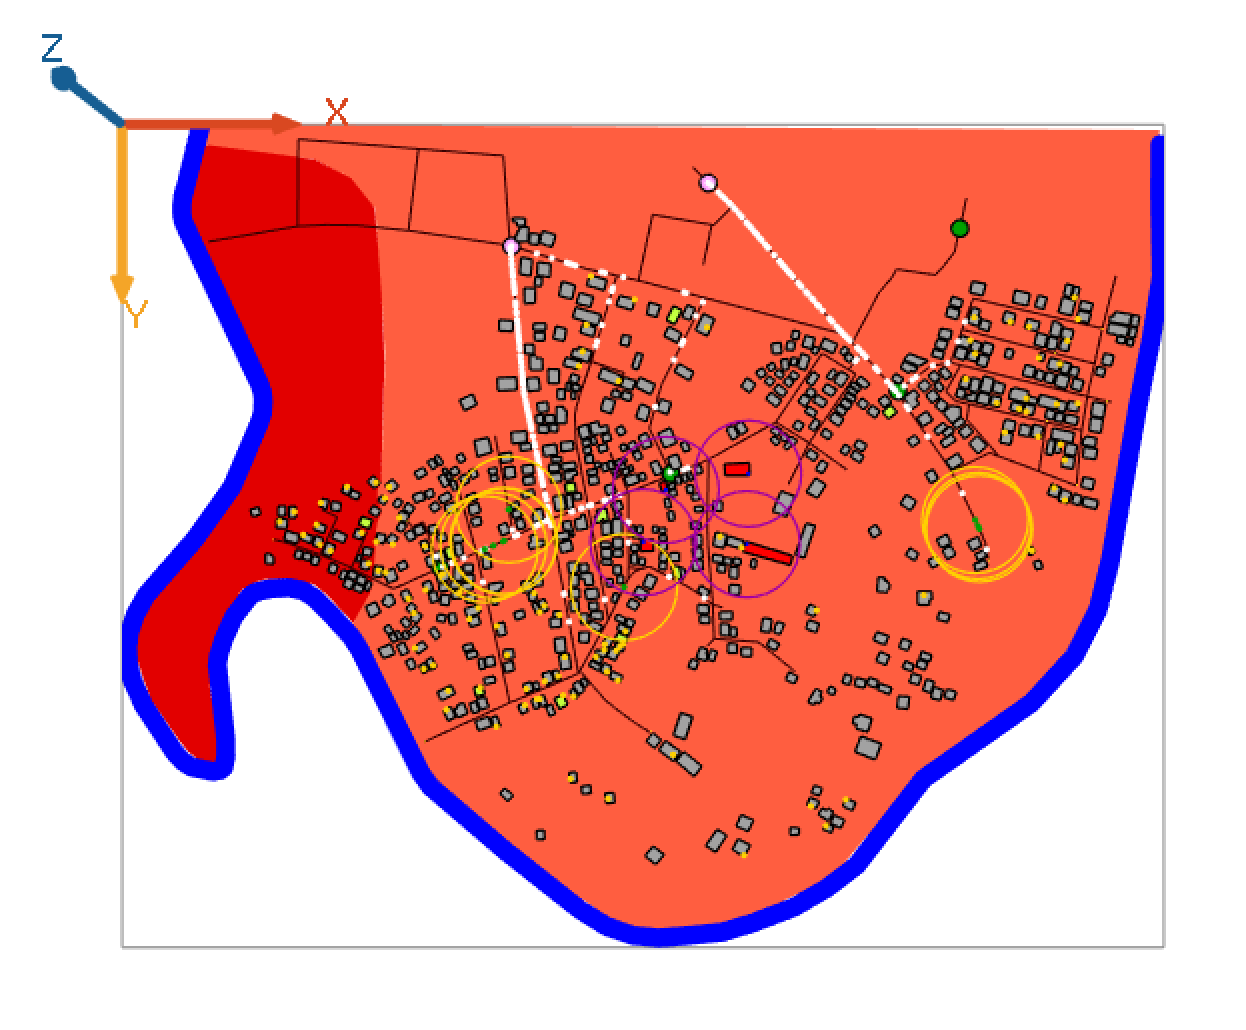
\includegraphics[width=\textwidth]{evacuationFullcap.png}
\caption{A figure caption is always placed below the illustration.
Please note that short captions are centered, while long ones are
justified by the macro package automatically.} \label{fig1}
\end{figure}

% \begin{theorem}
% This is a sample theorem. The run-in heading is set in bold, while
% the following text appears in italics. Definitions, lemmas,
% propositions, and corollaries are styled the same way.
% \end{theorem}

%
% the environments 'definition', 'lemma', 'proposition', 'corollary',
% 'remark', and 'example' are defined in the LLNCS documentclass as well.
%

\begin{proof}
Proofs, examples, and remarks have the initial word in italics,
while the following text appears in normal font.
\end{proof}

% ---- Bibliography ----
%
% BibTeX users should specify bibliography style 'splncs04'.
% References will then be sorted and formatted in the correct style.
%
% \bibliographystyle{splncs04}
% \bibliography{mybibliography}

\bibliographystyle{splncs04}
  \bibliography{sources}
\end{document}



% For citations of references, we prefer the use of square brackets
% and consecutive numbers. Citations using labels or the author/year
% convention are also acceptable. The following bibliography provides
% a sample reference list with entries for journal
% articles~\cite{szilagyi2000tool}, an LNCS chapter~\cite{ref_lncs1}, a
% book~\cite{ref_book1}, proceedings without editors~\cite{ref_proc1},
% and a homepage~\cite{ref_url1}. Multiple citations are grouped
% \cite{ref_article1,ref_lncs1,ref_book1},
% \cite{ref_article1,ref_book1,ref_proc1,ref_url1}.

% \begin{thebibliography}{8}
% \bibitem{ref_article1}
% Author, F.: Article title. Journal \textbf{2}(5), 99--110 (2016)

% \bibitem{ref_lncs1}
% Author, F., Author, S.: Title of a proceedings paper. In: Editor,
% F., Editor, S. (eds.) CONFERENCE 2016, LNCS, vol. 9999, pp. 1--13.
% Springer, Heidelberg (2016). \doi{10.10007/1234567890}

% \bibitem{ref_book1}
% Author, F., Author, S., Author, T.: Book title. 2nd edn. Publisher,
% Location (1999)

% \bibitem{ref_proc1}
% Author, A.-B.: Contribution title. In: 9th International Proceedings
% on Proceedings, pp. 1--2. Publisher, Location (2010)

% \bibitem{ref_url1}
% LNCS Homepage, \url{http://www.springer.com/lncs}. Last accessed 4
% Oct 2017
% \end{thebibliography}


